\documentclass[letter,12pt]{book}
\usepackage[spanish]{babel}
\usepackage[bookmarks]{hyperref}
\usepackage[utf8]{inputenc}
\usepackage{lmodern}
\usepackage{graphicx}
\usepackage{epstopdf}
\usepackage{pdflscape}
\usepackage{array}
\usepackage{apacite} 
\graphicspath{ {./imagenes/} }
\setcounter{secnumdepth}{3} % para que ponga 1.1.1.1 en subsubsecciones...
\setcounter{tocdepth}{3} % para que añada las subsubsecciones en el indice...

\begin{document}

  \begin{titlepage}

    \begin{center}
      \vspace*{-1in}
      \begin{figure}[htb]
    \begin{center}
      \includegraphics[width=8cm]{imagenes/Logo_Distrital.eps}
    \end{center}
    \end{figure}

    FACULTAD DE INGENIERÍA\\
    \vspace*{0.15in}
    PROYECTO CURRICULAR DE INGENIERÍA DE SISTEMAS \\
    \vspace*{0.6in}
    \begin{large}
    Tesis:\\
    \end{large}
    \vspace*{0.2in}
    \begin{Large}
    \textbf{EL TÍTULO DE LA TESIS} \\
    \end{Large}
    \vspace*{0.3in}
    \begin{large}
    Presentada por:\\
      Nicolás Mauricio Garcia Garzon 20091020031 \\
      Luis Felipe Gonzalez Moreno 20091020035
    \end{large}
    \vspace*{0.3in}
    \rule{80mm}{0.1mm}\\
    \vspace*{0.1in}
    \begin{large}
    Dirigida por: \\
    \end{large}
    \end{center}

    \end{titlepage}



  \newpage
  \mbox{}
  \thispagestyle{empty} % para que no se numere esta página
  
  
  \chapter*{Resumen} % si no queremos que añada la palabra "Capitulo"
  \addcontentsline{toc}{section}{Resumen} % si queremos que aparezca en el índice
  \markboth{RESUMEN}{RESUMEN} % encabezado
  
  \tableofcontents % indice de contenidos

  \cleardoublepage
  \addcontentsline{toc}{chapter}{Lista de figuras} % para que aparezca en el indice de contenidos
  \listoffigures % indice de figuras

  \cleardoublepage
  \addcontentsline{toc}{chapter}{Lista de tablas} % para que aparezca en el indice de contenidos
  \listoftables % indice de tablas
  
  \chapter{Definición del problema}
  El hombre, en su continua evolución, ha utilizado el lenguaje como una herramienta creadora de conocimiento transferible a sus congéneres o cualquier otro ser que interactuase con él. Con esto, “los humanos han desarrollado el lenguaje como un instrumento ligero y conveniente para mantener sus relaciones”\cite{dynamics}. 

En la comunicación entre congéneres, el lenguaje puede ser dividido en dos funciones: función de transmisión de información (gossip) y función de entendimiento del estado interno (estado mental) del congénere (mentalisation)\cite{dynamics}. Estas funciones de transmisión y entendimiento del otro han permitido que dos o varios humanos puedan asociarse entre sí formando redes sociales.

Las redes sociales no son otra cosa que la formación de lazos de algún tipo (emocional, de pertenencia a una comunidad, de trabajo, etc.) entre individuos que pueden ser organizaciones o humanos.\cite{sna_startups} En la figura \ref{fig:red_al_quaeda} puede verse cómo es representada la red social que forman las células terroristas de Al-Qaeda.

\begin{figure}[!htb]
  \begin{center}
    \includegraphics[width=11cm]{./imagenes/red_al_qaeda.png}
    \caption{Red social conformada por las células terroristas de Al-Qaeda.}
    \label{fig:red_al_quaeda}
  \end{center}
\end{figure}

La evolución de los servicios proporcionados a través de la internet ha sido drástica puesto que ha cambiado el modo de vida de las personas. En la figura \ref{fig:utilizacion_internet} se evidencia el crecimiento de la internet (de los servicios que en ella se soportan) se da en función de los servicios de conectividad social que son creados y soportados en ella. La web 1.0 fue utilizada en mayor medida por científicos para el intercambio de información en formato hipertexto. No había una interacción fuerte entre cada científico sino que ellos acudían a internet para buscar o poner a disposición material científico. Con la venida de la web 2.0 y la introducción de la interacción del usuario con la web generando contenido en tiempo real, así se crearon servicios de redes sociales en-línea (OSN en inglés: On-line Social Network), produciento una partición en los tipos de redes sociales. Así, las redes sociales a las que pertenece el ser humano en la era digital se dividieron convenientemente en “redes sociales fuera de línea” y redes sociales en línea (Offline Social Network y Online Social Network).

\begin{figure}[!htb]
  \begin{center}
    \includegraphics[width=11cm]{./imagenes/utilizacion_internet.png}
    \caption{Cambio de la utilización de internet en función de los servicios de conectividad social que son creados y soportados en ella}
    \label{fig:utilizacion_internet}
  \end{center}
\end{figure}

Las redes sociales fuera de línea son las redes sociales que se forman por comunicación tradicional (lenguaje oral y escrito en medios que difieran de aquellos que utilizan las telecomunicaciones). Las redes sociales en línea son aquellas redes sociales que están formadas por cibernautas y en las cuales la comunicación se da por medio de los servicios de redes sociales.

La administración de una red social fuera de línea fue estudiada desde inicios del siglo XX\cite{dynamics} con un enfoque socio-matemático llamado “análisis de redes sociales” (SNA por sus siglas en ingles: Social Network Analisis). Sin embargo, era difícil el análisis del comportamiento humano según los designios de la SNA puesto que la información debía ser recopilada por medio de entrevistas a las personas. Aún así, el enfoque SNA fue utilizado para analizar el comportamiento terrorista o inclusive el comportamiento de trabajadores en una empresa.\cite{sna_startups}

Con la creación de las OSN y la gran cantidad de información que describe el comportamiento humano sobre este tipo de red social, ha sido más sencillo utilizar el enfoque de la SNA para estudiar que comportamientos tienen los humanos sobre una red social establecida.

Los servicios de redes sociales (SNS por sus siglas en ingles: Social Network Services) como Facebook, LinkedIn, Twitter, SportTracker o Xportia, ofrecen servicios para la gestión de la OSN de cada usuario que acceda a estas aplicaciones. Según un estudio hecho para medir la experiencia de usuario (UX por sus siglas en ingles: User eXperience) en los SNS, se encontraron 8 categorías que son críticas a la hora de diseñar una SNS y son:

1. Self-expresion: Capacidad que tengan las OSN de compartir contenido relacionado a la vida real de los usuarios tal como lo pueden ser las fotos, los videos, los comentarios o las comunicaciones directas.
2. Reciprocity: Interacción bilateral en tiempo real, es decir, interacción instantánea con uno o varios individuales en la OSN (por ejemplo, por medio de los servicios de mensajería instantánea).
3. Learning: La información recibida por medio de la OSN debe poder ser utilizada en pro del desarrollo cognitivo del individual; debe existir información útil al individual que usa la OSN.
4. Curiosity: El contenido de la OSN debe ser interesante para quien la utiliza.
5. Suitability of functionality: Se refiere a cuán “utilizable” es una funcionalidad.
6. Suitability of content: La calidad y exactitud de la información que en la OSN reside debe ser suficiente para el individual perteneciente a ella.
7. Completeness of the user network: Los individuales deben querer pertenecer a la red social y buscar eficientemente a otros individuales para poder formar lazos con ellos y hacer crecer su red social.
8. Trust and privacy: Confianza en los servicios de las OSN, así como también la capacidad que tiene el usuario de gestionar la privacidad del contenido que comparte en dicha OSN.\cite{social_experience}

De acuerdo al enfoque SNA, las redes sociales pueden estar divididas en clusters, que no son más que agrupaciones de individuales sobre una red social por algún concepto como, por ejemplo, la pertenencia a una comunidad. Con lo anterior, podemos encontrar que algunos SNS ofrecen servicios para gestionar las OSN de sus usuarios centrándose en algún tipo de comunidad en específico y, la información que circula por ese tipo de comunidades, es diferente a la que pasa por SNS descentralizados (como Facebook y twitter). Viendo Facebook como una agrupación de clusters con temáticas tan diferentes como lo son los deportes y la música, la ciencia y la vida cotidiana, se puede decir que algunos SNS se enfocan en alguna de estas temáticas. En este caso, el cluster o temática que compete al trabajo a elaborar es el deporte.

Es posible hacer una división del cluster deporte en otros subclusters de cada uno de los deportes que existen en el mundo o en la clasificación de los deportes que han dado organizaciones como, por ejemplo, la IWGA (Internation WorldGames Association). Lo que se quiere con este trabajo es aportar al crecimiento de las redes sociales fuera de linea de las personas que practiquen deporte sin importar si lo hacen a nivel profesional o aficionado por medio de un SNS orientado a los deportes en general y, por lo tanto, el cluster que se ha escogido para trabajar es el del deporte como cluster mismo.

Se investigó acerca de las redes sociales existentes enfocadas a la temática del deporte y se encontró que muchas de ellas son utilizadas en mayor medida en España y que todas ellas están soportadas sobre tecnologías web. En general, solo se encontraron dos redes sociales deportivas orientadas a cualquier deporte asociadas a aplicaciones para smartphones disponibles en el la tienda virtual de Android o en la tienda virtual de Apple (La red social de Fitivity y Huddlers).

Así, con la evolución de la comunicación humana trasladándose a los espacios virtuales por medio de las OSN y la falta de aplicaciones, en el campo de los smartphones, que soporten interacciones sociales enfocadas a los deportes en general, en este trabajo se creará un SNS centrado en los deportes sobre tecnologías Android para la administración de las OSN de cada persona en un ámbito deportivo desde su dispositivo móvil.

  
  \chapter{Justificación del problema}
  Los humanos, desde siempre en su evolución, han necesitado de mecanismos para comunicarse con sus congéneres. En la actualidad, uno de los mecanismos es el uso de los SNS como facebook y twitter, cada uno de ellos modificando la forma de creación de redes sociales en la actualidad. (Sección \ref{sec:red})

De acuerdo al análisis egocéntrico de las redes sociales de cada individuo, se hace conveniente la utilización de SNS para gestionar las relaciones que un individuo mantiene con otros individuos (sean personas u organizaciones) en los diferentes círculos sociales en los que se mueve. (Sección \ref{sec:egocentrico})

El círculo social o comunidad escogida para el desarrollo propuesto es la comunidad deportiva debido a que hay mucha información dispersa alrededor de internet que es ambigua y a veces inclusive errónea. A su vez, debido a que gran cantidad de deportes no han tenido una acogida grande alrededor del mundo, las comunidades que se mueven sobre uno de esos deportes son más cerradas y, por ende, pequeñas y con poca información para un público que salga de las fronteras de dichas comunidades cerradas. Lo que se quiere con este trabajo es aportar al crecimiento de las redes sociales de las personas que practiquen deporte sin importar si lo hacen a nivel profesional o aficionado por medio de un SNS orientado a los deportes en general.

Un factor de utilización masiva de las SNS es que éstas estén orientadas a un público en particular y aumenten su cobertura dependiendo de su alcance de masa crítica sobre una red social definida \cite{sna_startups}. Al construir, en principio, la red social deportiva enfocada en dos deportes en particular, la probabilidad de ganar la masa crítica es mayor y, por tanto, el SNS desarrollado puede volverse más útil con el tiempo.

La UX de los SNS (visto en la sección \ref{sec:UX}) es otro factor, debido a que juega un papel importante pues es esta la segunda carta de presentación de un SNS. Algunas de las características que evalúan los usuarios en cuanto a la UX no son suplidas por los SNS actuales – o al menos no parcialmente - , tres de ellas (fundamentales para la acogida de un nuevo SNS) son “curiosity, learning y completeness of the social network”. Así, habiendo analizado 19 SNS orientados al deporte (Tablas \ref{tab:comparacion_redes_1} a \ref{tab:comparacion_redes_5}), se concluyó que fallaban en alguna de las tres características mencionadas.

Tener en cuenta la población a quien va dirigido el SNS a desarrollar es otro factor de éxito. Según \cite{user_behavior_online}, entre los años de adolescencia y los 40 años de edad, las personas acuden con mayor interés al uso de los SNS; al ser la comunidad del deporte comprendida en su mayoría por personas entre la adolescencia y los 40 años, aumenta aún más la probabilidad de alcanzar la masa crítica y volver útil con el tiempo el SNS.

Un último factor, que se observó, afecta la creación de redes sociales (tanto fuera de línea como en línea) (Sección \ref{sec:red}) es la distancia entre cada individual y el posible tipo de enlace que los uniría. Al ver la importancia de manejar SNS que ofrezcan servicios de geolocalización, se ha visto pertinente añadir dicho servicio a la creación del prototipo de SNS orientado a los deportes en general.

También se encontró evidencia de poca utilización de los SNS que no estaban orientadas a móviles. Dichos SNS eran utilizados mucho más por personas
que practican deportes que empiezan a tomar vuelo o deportes poco conocidos (un ejemplo de ello es el padel). El problema con dichos SNS es la
naturaleza nómada de los deportistas. Una solución a la naturaleza nómada de los deportistas y el acercamiento de los últimos a las TICs y, en este caso, a
los SNS deportivos es la aparición y utilización en masa de los smartphones.

En general, solo se encontraron dos redes sociales deportivas orientadas a cualquier deporte asociadas a aplicaciones para smartphones disponibles en el la tienda virtual de Android o en la tienda virtual de Apple (La red social de Fitivity y Huddlers) (Tablas \ref{tab:comparacion_redes_1} a \ref{tab:comparacion_redes_5}). Además, hay una ventaja real en hacer una red social orientada a dispositivos móviles y es la capacidad de movilidad que ellos brindan mientras se está utilizando el servicio \cite{spiderweb}. Dada la falta de aplicaciones móviles en el campo descrito y a su vez la importancia que toman los dispositivos móviles por sus características, se ha decidido hacer el prototipo de SNS orientado al deporte sobre tecnologías móviles.

  
  \chapter{Objetivos}
  \section{Objetivo General}
   Desarrollar un prototipo SNS (Social Networking Service) centrado en el deporte, sobre tecnologías Android, que permita al usuario el acceso a diferentes servicios propios de una red social con el fin de fortalecer a las comunidades que practican deporte, y a quienes quieren ser parte de ellas, facilitando la comunicación y el acceso a la información a los usuarios de la red.

  \section{Objetivos específicos}
   \begin{itemize}
  \item Investigar acerca de la teoría de las redes sociales, la computación orientada a servicios y el estado del arte de las redes sociales, con el fin de que el prototipo a desarrollar esté cimentado sobre bases teóricas sólidas.
  \item Identificar, analizar y evaluar las necesidades de la comunidad deportiva concernientes al SNS a implementar y, posteriormente, postular requerimientos funcionales y no funcionales para el SNS.
  \item Formular una arquitectura híbrida bajo el paradigma SOA que cumpla los diferentes requerimientos del proyecto, con el fin de tener un marco de trabajo que soporte cada etapa posterior a la formulación de esta.
  \item Postular, escoger y diseñar los servicios que darán solución a los requerimientos y necesidades identificadas para la implementación de la SNS, con el fin de gestionar cada incremento del proyecto y escoger los servicios a diseñar.
  \item Implementar y probar los diferentes servicios con el fin de cumplir los requerimientos planteados en la fase de análisis.
\end{itemize}

  
  \chapter{Marco teórico}
  
  \section{Redes Sociales}

\subsection{¿Qué es una red?}

Una red es un conjunto de relaciones. Mas específicamente, una red consiste en un conjunto de objetos (nodos) que están interconectados a través de relaciones (aristas). La red mas simple consiste en 2 nodos, N1 y N2, que están relacionados entre sí (Figura \ref{fig:simple}). Los nodos podrían representar personas, mientras la arista representa la relación que existe entre ellas (N1 y N2 son amigos, por ejemplo).

\begin{figure}[!htb]
  \begin{center}
    \includegraphics{./imagenes/Red_simple.eps}
    \caption{La red mas simple}
    \label{fig:simple}
  \end{center}
\end{figure}

Las relaciones pueden ser simétricas o asimétricas. Cuando se tiene una relación simétrica se dice que la relación no tiene dirección, es decir, la relación puede leerse en ambos sentidos. En el ejemplo anterior, significaría que N1 es amigo de N2 y que N2 es amigo de N1. Para que una relación se considere asimétrica, la relación debe poder leerse en un único sentido, es decir, la relación tiene una dirección determinada. En la figura \ref{fig:asimetrica} se puede observar un ejemplo de una red asimétrica en donde el nodo (o persona) N1 sigue al nodo N2, pero el nodo N2 no sigue al nodo N1.

\begin{figure}[!htb]
  \begin{center}
    \includegraphics{./imagenes/Red_asimetrica.eps}
    \caption{Ejemplo de una red asimetrica}
    \label{fig:asimetrica}
  \end{center}
\end{figure}

Es posible que exista mas de una relación entre 2 nodos, en ese caso se dice que existe una \textit{relación multiplex}

\subsection{Grado de centralidad}

En todas las redes, sean virtuales o no, existen personas que son mas ``importantes" que otras, más \textbf{populares}. Estas celebridades representan una parte muy pequeña de la red, pero debido a su gran influencia siempre es bueno identificarlos. Para esto se utiliza el \textbf{grado de centralidad}.

El grado de un nodo es la cantidad de conexiones que posee. En una red social, esto se representa por medio de las relaciones que cada nodo tenga, y ya que el significado de la relación varia en función de cada red, es necesario entender que significan las posibles relaciones existentes en una red para hacer el análisis correspondiente. Por ejemplo, en una red como Twitter en donde las relaciones son unidireccionales, puede existir un nodo con un grado de salida muy alto, esto es una persona que sigue a muchas otras. Aunque esta persona tenga un grado de centralidad muy alto, no representa una celebridad, sin embargo, un nodo que tenga un grado de entrada muy alto, que es seguido por muchas personas, si representa una persona que es muy popular en esta red.

\begin{figure}[!htb]
  \begin{center}
    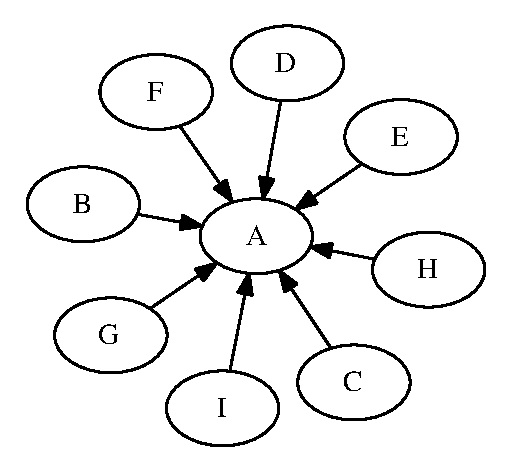
\includegraphics{./imagenes/red_estrella.eps}
    \caption{Red de estrella}
    \label{fig:red_estrella}
  \end{center}
\end{figure}

En la figura \ref{fig:red_estrella} se puede ver un caso en el que el nodo A es una clara celebridad de la red. Este tipo de configuración, llamada red de estrella, es muy poco común en la vida real, pero sirve de ayuda visual para entender a simple vista el concepto de centralidad.

\subsection{Grado de cercanía}

A menudo se puede ver que personas que no tienen mayor influencia aparente en una red son capaces de difundir un mensaje en una gran parte de la red. Esto se debe a que tienen buenas conexiones en la red que les permiten llegar a mas personas, sin que ellos en si sean ``importantes" en la red. Para medir que tan bien o mal posicionado esta un nodo en la red se utiliza el \textbf{grado de cercanía}. Este calculo es bastante caro computacionalmente ya que conlleva una gran cantidad de cálculos.

Los pasos para calcular el grado de cercanía de los nodos de una red son:

\begin{enumerate}
  \item Calcular la ruta mas corta entre todos los pares de nodos posibles, utilizando el algoritmo de Dijkstra, y almacenar estos valores en una tabla.
  \item Para cada nodo de la red:
  \begin{enumerate}
    \item Calcular la distancia promedio con todos los demás nodos.
    \item Dividir el promedio por la distancia mas alta.
    \item Calcular el inverso del valor anterior.
  \end{enumerate}
  \item normalizar cada valor obtenido para obtener valores en el rango de 0-1.
\end{enumerate}

Los nodos que tengan un valor mas cercano a 1 son los que tienen una distancia promedio menor con los nodos de la red, o los que tienen ``\textit{mejores contactos}".

\subsection{Grado de intermediación}

En las redes sociales, suelen formarse grupos mas pequeños que comparten un interés común. Por ejemplo, es mas probable que dos personas que comparten el gusto por los videojuegos interactúen entre si que dos personas que no lo hagan, sin embargo hay casos en los que una persona comparte gustos con diferentes grupos, ayudando a que esta persona se pueda relacionar de manera efectiva con un grupo mas extenso de personas. Estas personas son conocidas como ``puertas frontera" ya que, gracias a ellos, es posible que dos grupos que no tengan nada en común puedan relacionarse entre sí. La medida que ayuda a identificar estos elementos en una red es el \textbf{grado de intermediación}, y consiste en lo siguiente:

\begin{enumerate}
  \item Calcular la ruta mas corta entre todos los pares de nodos posibles, utilizando el algoritmo de Dijkstra, y almacenar estos valores en una tabla.
  \item Para cada nodo n de la red, contar las veces que el nodo n aparece en la lista de rutas mas cortas,
  \item normalizar cada valor obtenido para obtener valores en el rango de 0-1.
\end{enumerate}

Cabe notar que este algoritmo es bastante lento para redes que son muy grandes.

En la figura \ref{fig:bow_tie} se puede ver un claro ejemplo de este fenómeno. Esta red, conocida como la red corbatín (bow-tie en inglés), muestra como el nodo D se encuentra entre 2 grupos de nodos que, de otra manera, no podrían conectarse.

\begin{figure}[!htb]
  \begin{center}
    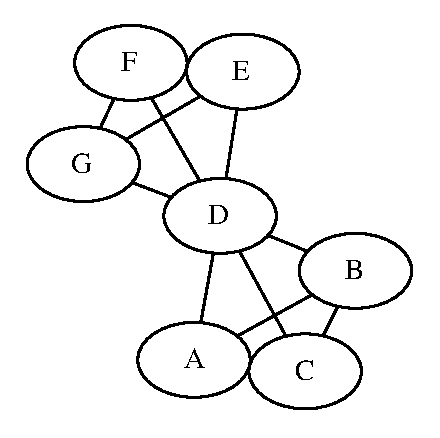
\includegraphics{./imagenes/bow_tie.eps}
    \caption{red corbatín}
    \label{fig:bow_tie}
  \end{center}
\end{figure}

\subsection{Díadas}

Las díadas son la unidad básica de análisis una red social, ya que estas representan la relación entre una y otra persona, esto es, mis amigos, mis seguidores, mis suscriptores, etc. Existen 4 tipos de díadas, representadas en la figura \ref{fig:tipos_diadas}, su uso varia en función del significado de la relación.

\begin{figure}[!htb]
  \begin{center}
      \begin{tabular}{m{3cm}|m{3cm}|m{3cm}|m{3cm}}
        \includegraphics[width=3cm]{./imagenes/diada_1.eps} & 
        \includegraphics[width=3cm]{./imagenes/diada_2.eps} & 
        \includegraphics[width=3cm]{./imagenes/diada_3.eps} & 
        \includegraphics[width=3cm]{./imagenes/diada_4.eps}\\
      \end{tabular}
    \caption{Tipos de diadas asimétricas}
    \label{fig:tipos_diadas}
  \end{center}
\end{figure}

La díada 1 indica que ambos individuos existen en la red, pero todavía no existe ninguna relación entre ellos. Las diadas 2 y 3 muestran una relación unidireccional entre los dos individuos, la única diferencia es el sentido de esa relación. La díada 4, por su parte, es la de mayor interés de las cuatro ya que muestra una relación bidireccional entre los individuos, siendo esta la relación que mayor peso tiene en una red social dado que nos dice que existe un alto grado de reciprocidad en el intercambio de información entra ambos individuos.

\subsection{Tríadas}

Las triadas son básicamente 3 nodos conectados de alguna manera. Al igual que con las diadas, las triadas también pueden ser simétricas o asimétricas, dependiendo estrictamente del contexto en que son utilizadas. Existen 4 tipos de triadas simétricas, ilustradas en la figura \ref{fig:tipos_triadas_simetricas}.

\begin{figure}[!htb]
  \begin{center}
      \begin{tabular}{m{3cm}|m{3cm}|m{3cm}|m{3cm}}
        \includegraphics[width=3cm]{./imagenes/triada_simetrica_1.eps} & 
        \includegraphics[width=3cm]{./imagenes/triada_simetrica_2.eps} & 
        \includegraphics[width=3cm]{./imagenes/triada_simetrica_3.eps} & 
        \includegraphics[width=3cm]{./imagenes/triada_simetrica_4.eps}\\
      \end{tabular}
    \caption{Tipos de triadas simétricas}
    \label{fig:tipos_triadas_simetricas}
  \end{center}
\end{figure}

Por otra parte, existen 16 tipos de triadas asimétricas, numeradas del 1-16. Su uso es mas frecuente ya que de ellas se puede hacer un análisis mas complejo en comparación a las díadas. Cada una de estas triadas recibe un nombre especifico para facilitar su identificación, a continuación se explica como debe leerse ese nombre:

\begin{itemize}
  \item El primer numero representa la cantidad de vértices bidireccionales
  \item El segundo numero representa la cantidad de vértices simples
  \item El tercer numero representa la cantidad de vértices inexistentes
  \item Si una triada se repite, se utiliza una letra extra para determinar que variante es:
  \begin{itemize}
    \item U - Arriba (Up)
    \item D - Abajo (Down)
    \item C - Circulo (Circle)
    \item T - Transitiva (Transitive)
  \end{itemize}
\end{itemize}

En la figura \ref{fig:tipos_triadas_asimetricas} se muestran todas las triadas posibles con su respectivo código asociado.

\begin{figure}[!htb]
  \begin{center}
      \begin{tabular}{m{1.3cm}|m{1.3cm}|m{1.3cm}|m{1.3cm}|m{1.3cm}|m{1.3cm}|m{1.3cm}|m{1.3cm}}
        \includegraphics[width=1.3cm]{./imagenes/triada_003.eps} & 
        \includegraphics[width=1.3cm]{./imagenes/triada_012.eps} & 
        \includegraphics[width=1.3cm]{./imagenes/triada_021C.eps} & 
        \includegraphics[width=1.3cm]{./imagenes/triada_021D.eps} & 
        \includegraphics[width=1.3cm]{./imagenes/triada_021U.eps} & 
        \includegraphics[width=1.3cm]{./imagenes/triada_030C.eps} & 
        \includegraphics[width=1.3cm]{./imagenes/triada_030T.eps} & 
        \includegraphics[width=1.3cm]{./imagenes/triada_102.eps}\\ \hline
        \includegraphics[width=1.3cm]{./imagenes/triada_111D.eps} & 
        \includegraphics[width=1.3cm]{./imagenes/triada_111U.eps} & 
        \includegraphics[width=1.3cm]{./imagenes/triada_120C.eps} & 
        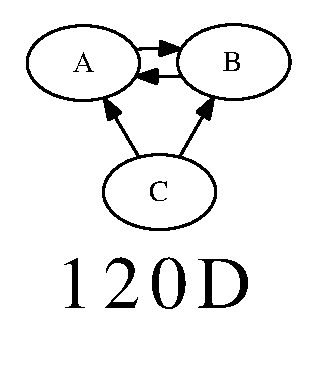
\includegraphics[width=1.3cm]{./imagenes/triada_120D.eps} & 
        \includegraphics[width=1.3cm]{./imagenes/triada_120U.eps} & 
        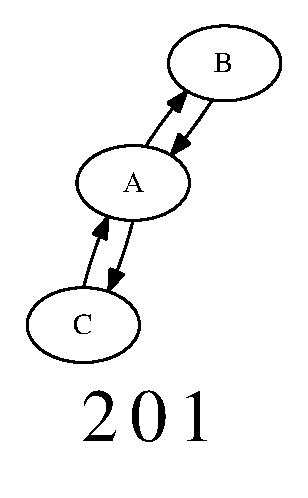
\includegraphics[width=1.3cm]{./imagenes/triada_201.eps} & 
        \includegraphics[width=1.3cm]{./imagenes/triada_210.eps} & 
        \includegraphics[width=1.3cm]{./imagenes/triada_300.eps}\\
      \end{tabular}
    \caption{Tipos de triadas asimétricas}
    \label{fig:tipos_triadas_asimetricas}
  \end{center}
\end{figure}

Gracias a esta discriminación topológica, se puede hacer un análisis mas completo de una red. Este análisis recibe el nombre de \textbf{\textit{Análisis Triadico}}.

\subsection{Análisis Triadico}

Este proceso, que también recibe el nombre de \textbf{Censo Triadico}, consiste en contar la ocurrencia de cada uno de los tipos de triada para cada nodo, y de esa forma determinar el rol que desempeña este nodo en la red. Por ejemplo, un nodo que presente en mayoría triadas del tipo 4, 7 y 11 es un nodo que \textbf{genera contenido}, mientras que si la mayoría de sus triadas son del tipo 5 y/o 10, es un nodo que recibe o \textbf{consume contenidos}.

Adicionalmente se puede hacer el mismo análisis a la red en general, para tener un punto de vista global de la red. En la figura \ref{fig:red_krackhardt} se puede ver una de las redes mas utilizadas en la teoría de redes sociales, la red de Krackhardt-kite. En esta red se pueden ver muchas características de una red social, facilitando el estudio de las mismas. Al hacer el censo a esta red, nos damos cuenta que presenta una gran cantidad de nodos tipo 201, que representan un agujero estructural, y nodos tipo 300, que representan triadas cerradas, esto nos indica que en esta red existen zonas que tienen una gran concentración de nodos interconectados, mientras hay zonas que no se encuentran muy pobladas. Todo esto se puede ver a simple vista en esta red, pero para redes mas grandes puede que represente un problema mayor.

\begin{figure}[!htb]
  \begin{center}
    \includegraphics[width=8cm]{./imagenes/red_krackhardt_kite.eps}
    \caption{Red social de Krackhardt kite}
    \label{fig:red_krackhardt}
  \end{center}
\end{figure}

\subsection{Pandillas}


\input{./Capitulos/4-Marco_teorico/BPMN.tex}

\section{Service-Oriented Architecture (SOA)}
\subsection{Proceso de Análisis y diseño orientados a servicios}

En la etapa de análisis y diseño, el arquitecto de software se reúne con un analista de negocio, el cual diseñará unos servicios candidatos que después se convertirán en los servicios incluidos en los blueprints. Luego de tener los planos, el arquitecto escoge un subconjunto de dichos candidatos a servicios para ser implementados físicamente, dotándolos de algún método para realizar la composición de servicios. En la figura \ref{fig:seis} se muestra el proceso de análisis y diseño orientado a servicios.

\begin{figure}[!htb]
  \begin{center}
    \includegraphics[width=11cm]{./imagenes/6.png}
    \caption{proceso de análisis y diseño orientado a servicios}
    \label{fig:seis}
    \textbf{Fuente:}  \cite{soa_principles}
  \end{center}
\end{figure}

\subsection{Metas y beneficios de la computación orientada a servicios }

Las metas y los beneficios que trae la implementación de la computación orientada a servicios en una organización son:

\begin{itemize}
  \item \textbf{Incremento de la interoperabilidad intrínseca}: Es una meta de la computación orientada a servicios ya que la composición de servicios requiere que, sin necesidad de integrar un servicio con el otro, estos puedan intercambiar información para desarrollar la funcionalidad a la que han sido inscritos. Aplicando principios de diseño orientados a servicios, así como también estándares de diseño orientados a servicios, se logra el incremento de la interoperabilidad intrínseca.
  \item \textbf{Federación incrementada}: Un entorno de TI federado es aquel en el cual los recursos y aplicaciones se manejan y gobiernan con autonomía y por sí mismos. En el ámbito de la orientación a servicios, cada servicio puede tener su propia implementación independiente y aun así comunicarse. Esto se logra por medio de una especial atención a los estándares de diseño.
  \item \textbf{Incremento de opciones en la escogencia de proveedores de servicios}: Como la federación en la computación orientada a servicios es una meta, la escogencia de proveedores de servicios diferentes es un beneficio ya que la composición de servicios puede ser lograda sin importar que proveedor provea de un servicio específico.
  \item \textbf{Incremento de la alineación entre el negocio y las tecnologías}: Ya que en el proceso de diseño actúan tanto el analista de negocio como el arquitecto de software, la alineación entre negocio y tecnologías es incrementada. La reconfiguración en la composición de servicios, además, provee alineación extra al poder cambiar el proceso de negocio y la composición de los servicios al mismo tiempo.
  \item \textbf{ROI}: Al hacerse inventarios de servicios y, además, ser los servicios reutilizables a lo largo del tiempo y compuestos de diferente forma gracias a la composición de servicios, se da una relación costo/beneficio más baja que con otros paradigmas usados.
  \item \textbf{Agilidad organizacional incrementada}: Debido a la orientación a servicios, se hace una composición rápida de los servicios que se tengan y se crean los que se necesiten para agilizar el proceso del departamento de TI y así agilizar los procesos subyacentes.
  \item \textbf{Reducción de cargas al departamento TI}: Debido a la agilidad organizacional cuando es aplicada la orientación a servicios, son reducidos costos operacionales (tiempo u otros recursos) y el departamento de TI adquiere un papel activo en el sector estratégico.
\end{itemize}


\section{Estado del arte} \label{cap:estado_arte}
\subsection{UX - Análisis}
Los servicios de redes sociales (SNS por sus siglas en ingles: Social Network Services) como Facebook, LinkedIn, Twitter, SportTracker o Xportia, ofrecen servicios para la gestión de la OSN de cada usuario que acceda a estas aplicaciones. Según un estudio hecho para medir la experiencia de usuario (UX por sus siglas en ingles: User eXperience) en los SNS, se encontraron 8 categorías que son críticas a la hora de diseñar una SNS y son:

\begin{enumerate}
  \item Self-expresion: Capacidad que tengan las OSN de compartir contenido relacionado a la vida real de los usuarios tal como lo pueden ser las fotos, los videos, los comentarios o las comunicaciones directas.
  \item Reciprocity: Interacción bilateral en tiempo real, es decir, interacción instantánea con uno o varios individuales en la OSN (por ejemplo, por medio de los servicios de mensajería instantánea).
  \item Learning: La información recibida por medio de la OSN debe poder ser utilizada en pro del desarrollo cognitivo del individual; debe existir información útil al individual que usa la OSN.
  \item Curiosity: El contenido de la OSN debe ser interesante para quien la utiliza.
  \item Suitability of functionality: Se refiere a cuán ``utilizable'' es una funcionalidad.
  \item Suitability of content: La calidad y exactitud de la información que en la OSN reside debe ser suficiente para el individual perteneciente a ella.
  \item Completeness of the user network: Los individuales deben querer pertenecer a la red social y buscar eficientemente a otros individuales para poder formar lazos con ellos y hacer crecer su red social.
  \item Trust and privacy: Confianza en los servicios de las OSN, así como también la capacidad que tiene el usuario de gestionar la privacidad del contenido que comparte en dicha OSN. \cite{social_experience}

Cada uno de las categorías nombradas hace parte de los factores que impulsan la utilización de los SNS para la gestión de las OSN de las personas. 
\end{enumerate}

\subsection{Factor distancia en la formación de las redes sociales}

La formación de redes sociales (tanto fuera de línea como en línea) es afecta por la distancia entre cada individual y el posible tipo de enlace que los uniría. En \cite{evolution} se hizo un estudio acerca de la formación de lazos, la formación de triadas entre individuales de una red social basada en la inscripción localizaciones recomendadas y frecuentadas por los usuarios, teniendo como parámetros ``la edad'' o tiempo de vinculación del individual a la red social, el grado de cada individual (número de conexiones que tiene un individual a otro) y la localización de cada individual en la red social. También se analizó cómo afectaba la creación de nuevos lazos con la movilidad del usuario (el desplazamiento por lugares geográficos distintos). En conclusión, se verificó que la formación de lazos depende proporcionalmente de la edad y del grado del individual y es inversamente proporcional a la distancia que a cada individual y que la formación de lazos puede modelarse con solo dos de los tres factores (el grado y la distancia); en cuanto a la formación de triadas, se verificó que ésta depende de las características sociales de la red, tomando énfasis en los individuales compartidos entre los posibles individuales formadores de triadas. Además, en cuanto a la creación de nuevos lazos teniendo en cuenta los lugares visitados por cada usuario de la red social, se presenta un patrón: Los usuarios escogen un lugar popular para visitar y, posteriormente, dirimen con que usuario crear un lazo teniendo en cuenta su popularidad y que frecuente los mismos lugares siempre.

\begin{landscape}
  
\begin{table}
  \caption{Comparacion de redes, parte 1}
  \label{tab:comparacion_redes_1}

  \begin{center}
  
  \resizebox{20cm}{!}{
  \begin{tabular}{|p{5cm}|llll|}
    \hline
    Fun\textbackslash Red social & \multicolumn{1}{c}{Sportfactor} & \multicolumn{1}{c}{Deportesreunidos} & \multicolumn{1}{c}{Mybestplay} & \multicolumn{1}{c|}{Subetudeporte} \\ 
    \hline
    Gestión de foros & \multicolumn{1}{c}{} & \multicolumn{1}{c}{Si} & \multicolumn{1}{c}{} & \multicolumn{1}{c|}{Si} \\ 
    \hline
    Gestión de encuentros deportivos & \multicolumn{1}{c}{} & \multicolumn{1}{c}{- Organización de eventos} & \multicolumn{1}{c}{} & \multicolumn{1}{c|}{} \\ 
     & \multicolumn{1}{c}{} & \multicolumn{1}{c}{-Encuentros deportivos informales} & \multicolumn{1}{c}{} & \multicolumn{1}{c|}{} \\ 
     & \multicolumn{1}{c}{} & \multicolumn{1}{c}{} & \multicolumn{1}{c}{} & \multicolumn{1}{c|}{} \\ 
    \hline
    Creación de grupos & \multicolumn{1}{c}{} & \multicolumn{1}{c}{Si} & \multicolumn{1}{c}{} & \multicolumn{1}{c|}{} \\ 
    \hline
    Manejo de torneos & \multicolumn{1}{c}{} & \multicolumn{1}{c}{- Organización y difusión} & \multicolumn{1}{c}{} & \multicolumn{1}{c|}{} \\ 
    \hline
    Difusión info. Deportiva & \multicolumn{1}{c}{-RSS de noticias} & \multicolumn{1}{c}{- Blog propio} & \multicolumn{1}{c}{-Difusión de eventos} & \multicolumn{1}{c|}{- Gestión de blogs} \\ 
     & \multicolumn{1}{c}{} & \multicolumn{1}{c}{} & \multicolumn{1}{c}{-Blog propio} & \multicolumn{1}{c|}{} \\ 
    \hline
    Serv. self-expression & \multicolumn{1}{c}{} & \multicolumn{1}{c}{-Difusión de multimedia} & \multicolumn{1}{c}{-Difusión de multimedia } & \multicolumn{1}{c|}{-Difusión de multimedia} \\ 
     & \multicolumn{1}{c}{} & \multicolumn{1}{c}{} & \multicolumn{1}{c}{} & \multicolumn{1}{c|}{} \\ 
    \hline
    Sistema estadístico & \multicolumn{1}{c}{-Medición de avance en} & \multicolumn{1}{c}{- Sistemas de estadísticas para cada servicio} & \multicolumn{1}{c}{} & \multicolumn{1}{c|}{} \\ 
     & \multicolumn{1}{c}{ estadísticas del deporte practicado} & \multicolumn{1}{c}{} & \multicolumn{1}{c}{} & \multicolumn{1}{c|}{} \\ 
    \hline
    Gestión de transversales & \multicolumn{1}{c}{-Trainner personales} & \multicolumn{1}{c}{} & \multicolumn{1}{c}{} & \multicolumn{1}{c|}{} \\ 
     & \multicolumn{1}{c}{-Guías de nutrición} & \multicolumn{1}{c}{} & \multicolumn{1}{c}{} & \multicolumn{1}{c|}{} \\ 
     & \multicolumn{1}{c}{- Catalogo de lesiones y fisioterapia} & \multicolumn{1}{c}{} & \multicolumn{1}{c}{} & \multicolumn{1}{c|}{} \\ 
    \hline
    Servicios deportivos & \multicolumn{1}{c}{-Guía deportiva (shops, restaurantes, etc.)} & \multicolumn{1}{c}{} & \multicolumn{1}{c}{} & \multicolumn{1}{c|}{} \\ 
     & \multicolumn{1}{c}{} & \multicolumn{1}{c}{} & \multicolumn{1}{c}{} & \multicolumn{1}{c|}{} \\ 
    \hline
    Soporte multi-deporte & \multicolumn{1}{c}{Si} & \multicolumn{1}{c}{Si} & \multicolumn{1}{c}{Solo deportes en equipo} & \multicolumn{1}{c|}{Si} \\ 
    \hline
    Gestión de tipos de usu. & \multicolumn{1}{c}{} & \multicolumn{1}{c}{- Equipos } & \multicolumn{1}{c}{Si} & \multicolumn{1}{c|}{} \\ 
     & \multicolumn{1}{c}{} & \multicolumn{1}{c}{- Clubes} & \multicolumn{1}{c}{} & \multicolumn{1}{c|}{} \\ 
     & \multicolumn{1}{c}{} & \multicolumn{1}{c}{-Centros deportivos} & \multicolumn{1}{c}{} & \multicolumn{1}{c|}{} \\ 
    \hline
    Gestión de sponsors & \multicolumn{1}{c}{} & \multicolumn{1}{c}{} & \multicolumn{1}{c}{Si} & \multicolumn{1}{c|}{} \\ 
    \hline
    Gestión del conocimiento & \multicolumn{1}{c}{} & \multicolumn{1}{c}{} & \multicolumn{1}{c}{} & \multicolumn{1}{c|}{} \\ 
    \hline
    Gestión de geolocaliza. & \multicolumn{1}{c}{} & \multicolumn{1}{c}{} & \multicolumn{1}{c}{} & \multicolumn{1}{c|}{} \\ 
     & \multicolumn{1}{c}{} & \multicolumn{1}{c}{} & \multicolumn{1}{c}{} & \multicolumn{1}{c|}{} \\ 
    \hline
    Soporte móvil & \multicolumn{1}{c}{} & \multicolumn{1}{c}{} & \multicolumn{1}{c}{} & \multicolumn{1}{c|}{} \\ 
     & \multicolumn{1}{c}{} & \multicolumn{1}{c}{} & \multicolumn{1}{c}{} & \multicolumn{1}{c|}{} \\ 
    \hline
    Conexión con otros SNS & \multicolumn{1}{c}{} & \multicolumn{1}{c}{} & \multicolumn{1}{c}{} & \multicolumn{1}{c|}{} \\ 
     & \multicolumn{1}{c}{} & \multicolumn{1}{c}{} & \multicolumn{1}{c}{} & \multicolumn{1}{c|}{} \\ 
    \hline
  \end{tabular}
  }
    \end{center}
\end{table}
  
  \newpage
  
  \begin{table}
  \caption{Comparacion de redes, parte 2}
  \label{tab:comparacion_redes_2}

  \begin{center}
  
  \resizebox{20cm}{!}{
    \begin{tabular}{|p{4cm}|p{9cm}p{7cm}p{7cm}|}
\hline
Fun\textbackslash Red social & Sporttia & Amatteur & Fitivity  \\ 
\hline
Gestión de foros &  &  &  \\ 
\hline
Gestión de encuentros deportivos & - Organización de eventos en centros deportivos & - Publicación o búsqueda de eventos deportivos & -Basado en geolocalización \\ 
 & - Gestión de jugadores &  &  \\ 
 & -Gestión de características del partido &  &  \\ 
\hline
Creación de grupos &  &  &  \\ 
\hline
Manejo de torneos &  &  &  \\ 
\hline
Difusión info. Deportiva &  &  &  \\ 
 &  &  &  \\ 
\hline
Serv. self-expression &  & -Difusión de multimedia &  \\ 
 &  &  &  \\ 
\hline
Sistema estadístico &  &  &  \\ 
 &  &  &  \\ 
\hline
Gestión de transversales &  &  &  \\ 
 &  &  &  \\ 
 &  &  &  \\ 
\hline
Servicios deportivos & -Alquiler de centros deportivos & - Servicios de compra y venta de artículos deportivos &  \\ 
 &  &  &  \\ 
\hline
Soporte multi-deporte & Si & Si & Si \\ 
\hline
Gestión de tipos de usu. & -Deportista -Centro deportivo & -Deportista  &  \\ 
 &  & -Equipo &  \\ 
 &  &  -Organización &  \\ 
\hline
Gestión de sponsors &  & -Promoción como deportista, equipo u organización &  \\ 
\hline
Gestión del conocimiento & - Clases virtuales &  &  \\ 
\hline
Gestión de geolocaliza. &  & Si & Si \\ 
 &  &  &  \\ 
\hline
Soporte móvil &  &  & -Android \\ 
 &  &  & -IOS \\ 
\hline
Conexión con otros SNS &  &  &  \\ 
\hline
\multicolumn{1}{l}{} &  &  & \multicolumn{1}{l}{} \\ 
\end{tabular}
  }
      \end{center}
\end{table}

\newpage

\begin{table}
  \caption{Comparacion de redes, parte 3}
  \label{tab:comparacion_redes_3}

  \begin{center}
  \resizebox{20cm}{!}{
  \begin{tabular}{|p{4cm}|p{7cm}p{6cm}p{9cm}|}
\hline
Fun\textbackslash Red social & Bkool & Deportmeet & Sportsnak \\ 
\hline
Gestión de foros &  &  & - Foros con profesionales (managers, coaches, teams) \\ 
 &  &  & - Ofrece posibilidad al usuario de ser moderador de foros \\ 
\hline
Gestión de encuentros deportivos & - Creación de eventos deportivos (solo o con amigos) &  - Gestión de eventos deportivos & - Manejo de eventos deportivos \\ 
 & - Gestión de ``retos'' &  &  \\ 
\hline
Gestión de grupos & Si &  &  \\ 
\hline
Manejo de torneos &  &  &  \\ 
\hline
Difusión info. Deportiva & - Gestión de información de ligas & - Artículos de profesionales & -Asociación con blogs deportivos \\ 
 &  &  & - Manejo de ``live scores'' \\ 
\hline
Serv. self-expression & -Subida de texto plano & -Difusión de multimedia & - Manejo contenido plano y multimedia \\ 
 & -Difusión de multimedia &  & - Uso de mensajería instantánea \\ 
\hline
Sistema estadístico & - Estadísticas de deportista & - Gestión del nivel del deportista &  \\ 
 &  & -Manejo de perfiles de usuario &  \\ 
\hline
Gestión de transversales &  & -Foros de nutrición &  \\ 
\hline
Servicios deportivos &  & - Venta de artículos deportivos & - Módulos para negociantes en temas de deporte \\ 
 &  &  & - Manejo de ofertas en ofrecimiento de instalaciones deportivas \\ 
 &  &  & -- Herramientas para hacer ``boost'' a negociantes (bussiness member) \\ 
\hline
Soporte multi-deporte & Deportes de ruta & Si & Si \\ 
 &  &  &  \\ 
\hline
Gestión de tipos de usu. &  &  & -Public member \\ 
 &  &  & -Club member \\ 
 &  &  & -Bussiness member \\ 
\hline
Gestión de sponsors &  &  & - Manejo de ``sponsorship'' \\ 
\hline
Gestión del conocimiento &  &  &  \\ 
 &  &  &  \\ 
\hline
Gestión de geolocaliza. & - Posibilidad de grabar trazados & - Localización de eventos & - Geolocalización de actividad deportiva cercana a un punto \\ 
 & (deportes de ruta) &  &  \\ 
\hline
Soporte móvil & -Android &  &  \\ 
 & -IOS &  &  \\ 
\hline
Conexión con otros SNS & -Facebook &  &  \\ 
 & -twitter &  &  \\ 
\hline
\end{tabular}
}
  
  \end{center}
\end{table}

\newpage

\begin{table}
  \caption{Comparacion de redes, parte 4}
  \label{tab:comparacion_redes_4}

  \begin{center}
    \resizebox{20cm}{!}{
    \begin{tabular}{|p{5cm}|lll|}
\hline
Fun\textbackslash Red social & Huddlers & Yoyde & Timpik \\ 
\hline
Gestión de foros &  &  &  \\ 
 &  &  &  \\ 
\hline
Gestión de encuentros deportivos & - Organización de eventos deportivos & - Manejo de eventos deportivos & - Manejo de eventos deportivos \\ 
 &  &  &  \\ 
\hline
Gestión de grupos &  &  &  \\ 
 &  &  &  \\ 
\hline
Manejo de torneos &  & Si &  \\ 
\hline
Difusión info. Deportiva &  & - Manejo de blogs &  \\ 
 &  &  &  \\ 
\hline
Serv. self-expression &  & -Manejo de ``muro'' & - Manejo de ``muro''  \\ 
 &  &  & -Gestión de mensajería \\ 
\hline
Sistema estadístico &  &  &  \\ 
 &  &  &  \\ 
 &  &  &  \\ 
\hline
Gestión de transversales &  &  &  \\ 
\hline
Servicios deportivos &  &  &  \\ 
\hline
Soporte multi-deporte & Si & Si & Si \\ 
 &  &  &  \\ 
\hline
Gestión de tipos de usu. &  & -Club deportivo & - Manejo de perfil deportivo \\ 
 &  & -Deportista &  \\ 
\hline
Gestión de sponsors &  &  &  \\ 
\hline
Gestión del conocimiento &  &  &  \\ 
 &  &  &  \\ 
\hline
Gestión de geolocaliza. & - Funcionalidad ``jugando en'' & - Manejo de escenarios deportivos &  \\ 
 &  & - Manejo de ``rutas'' &  \\ 
\hline
Soporte móvil & -IOS &  & -Android \\ 
\hline
Conexión con otros SNS &  &  &  \\ 
\hline
\end{tabular}
}
  
  \end{center}
\end{table}

\begin{table}
  \caption{Comparacion de redes, parte 5}
  \label{tab:comparacion_redes_5}

  \begin{center}
  \resizebox{20cm}{!}{
    \begin{tabular}{|p{4cm}|p{7cm}p{7cm}p{8cm}|}
\hline
Fun\textbackslash Red social & Socialsports & Strava & Ineftos \\ 
\hline
Gestión de foros &  &  & Si \\ 
\hline
Gestión de encuentros deportivos & - Organizador de eventos deportivos & - Manejo de desafíos (challenges) & - Organización de eventos \\ 
\hline
Gestión de grupos &  &  & Si \\ 
\hline
Manejo de torneos &  &  &  \\ 
\hline
Difusión info. Deportiva &  &  & - Manejo de blogs para estudiantes \\ 
\hline
Serv. self-expression & - Manejo de multimedia &  & - Manejo de mensajería \\ 
 &  &  & - Manejo de ``muro'' \\ 
 &  &  & - Manejo de multimedia \\ 
\hline
Sistema estadístico &  & - Gestión de estadísticas del atleta & - Utiliza mecanismo de encuestas para autorregularse \\ 
 &  & - Gestión de ``follows'' a otros deportistas para comparación de estadísticas (competencia) & - Gestión de foros: Estadísticas de foro \\ 
\hline
Gestión de transversales &  &  &  \\ 
\hline
Servicios deportivos & - Evaluación de la comunidad sobre los prestadores de servicio &  &  \\ 
\hline
Soporte multi-deporte & Si & Monodeporte (ciclomontañismo) & Si \\ 
\hline
Gestión de tipos de usu. & - Manejo de perfil de deportista (deportes practicados, lugares frecuentados, horarios frecuentados) &  & - Manejo de usuarios (profesores, alumnos, entidades sin ánimo de lucro) \\ 
 & - Manejo de usuarios (prestadores de servicio y deportistas) &  &  \\ 
\hline
Gestión de sponsors &  &  &  \\ 
\hline
Gestión del conocimiento &  & - Encuentro de consejos deportivos & - ``Social learning'' \\ 
\hline
Gestión de geolocaliza. &  & - Gestión de trazados logrados &  \\ 
 &  & - Gestión de trazados &  \\ 
\hline
Soporte móvil &  & -Android &  \\ 
\hline
Conexión con otros SNS &  &  &  \\ 
\hline
\end{tabular}
  }
  \end{center}
\end{table}

\end{landscape}


  
  \chapter{Metodología}
  
Equipo SCRUM:

\begin{itemize}
  \item Product Owner \\
	Doctor Carlos Enrique Montenegro

  \item Developement Team
	\begin{itemize}
	  \item Nicolás Mauricio García Garzón
	  \item Luis Felipe Gonzalez Moreno
	\end{itemize}

  \item Scrum Master \\
	Profesor Alejandro Daza
\end{itemize}

Actividades de cada Sprint (15 días máximo):
  
\begin{itemize}
  \item Sprint Planning (4 horas máximo)\\
  Se realizó una reunión con el Scrum Master al inicio de cada iteración. En esta reunión se discutió el desempeño del Sprint anterior, los servicios/funcionalidades que hacían falta para completar el prototipo, y que servicios debían ser realizados en la iteración.
	\begin{itemize}
	  \item ¿Qué se hizo en cada sprint? \\
	    Con base a los servicios y casos de uso de negocio encontrados, se determino que podía ser desarrollado por el developement team en cada iteración del prototipo.
	  \item ¿Como se llevará a cabo este trabajo? \\
	    Se dividieron los servicios propuestos como parte del Sprint entre los desarrolladores y se compartieron las expectativas que debe cumplir cada servicio para que sea aceptado en el desarrollo.
	\end{itemize}
  \item Daily Scrum (15 minutos máximo)[Solo participa el developement team] \\
  Partiendo de los items asignados a cada desarrollador, se dividieron en tareas aún mas pequeñas que sirvieron como ruta para cumplir con el Sprint Goal. Se respondieron las siguientes preguntas para llevar un seguimiento continuo del desarrollo del prototipo:
	\begin{itemize}
	  \item ¿Qué se hizo ayer que ayudó al developement team para cumplir el Sprint goal?
	  \item ¿Qué se va a hacer hoy para ayudar al developement team a cumplir el Sprint goal?
	  \item ¿Hay algún impedimento para que el developement team cumpla el Sprint goal?
	\end{itemize}
  \item Sprint Review (2 horas máximo) \\
  Se realizó al final de cada Sprint. Se mostro qué se hizo en el sprint con respecto a las tareas propuestas desde el inicio del mismo. Las actividades básicas que se llevaron a cabo fueron:
	\begin{itemize}
	  \item Socializar la experiencia en el sprint, que problemas ocurrieron y cómo se solucionaron.
	  \item Exponer los diferentes elementos que fueron construidos y se resuelven preguntas acerca de los mismos.
	  \item Proponer que puede hacerse en el siguiente Sprint basados en la experiencia del actual.
	  \item Revisar cómo el cambio en el entorno pudo cambiar las prioridades en el trabajo del equipo.
	\end{itemize}
  \item Sprint Retrospective
  \begin{itemize}
    \item Se tomaron las experiencias de cada sprint para formular sugerencias que ayudaron a mejorar los siguientes.

  \end{itemize}
\end{itemize}

A continuación, se presenta el product backlog inicial del proyecto.

\begin{table}[h]
  \caption{Product backlog inicial}
  \label{tab:backlog}

  \begin{center}
    \resizebox{15cm}{!}{
      \begin{tabular}{|l|l|l|}
        \hline
        Tarea & Días & Condición de aprobación \\ 
        \hline
        \hline
        Levantamiento de requerimientos & 2 & Satisfacción de todos los \\ 
        
         &  & requerimientos para la red social \\ 
        
        Definición de requerimientos funcionales y no funcionales & 2 & Modularización y descripción total de  \\ 
        
         &  & todos los requerimientos \\ 
        
        Investigación de tecnologías existentes & 6 & Escogencia de las tecnologías a utilizar \\ 
        
         &  & para implementar la red social \\ 
        
        Diseño de casos de uso & 5 & Cubrimiento de todos los requerimientos identificados \\ 
        
        Refinamiento de requerimientos & 1 & Trazabilidad entre casos de uso y requerimientos \\ 
        
        Identificación de servicios candidatos & 1 & Cubrimiento de todos los requerimientos identificados \\ 
        
        Diseño de blueprints de servicios & 4 & Cubrimiento de todos los servicios candidatos \\ 
        
        Escogencia de servicios a ser implementados & 1 & Viabilidad de un prototipo funcional \\ 
        
        Composición estática de servicios & 5 & Concordancia entre los casos de uso  \\ 
        
         &  & y la composición de servicios \\ 
        
        
        Diseño de base de datos & 6 & Diseño que cubra los servicios a ser implementados \\ 
        
         &  &  y requerimientos no funcionales \\ 
        
        Diseño de interfaz gráfica de usuario & 4 & Cubrimiento de los servicios y casos de uso a ser implementados \\ 
        
         &  &  a ser implementados \\ 
        
        Refinamiento de casos de uso & 1 & Trazabilidad \\ 
        
        Refinamiento de blueprints de servicios & 1 & Trazabilidad \\ 
        
        Refinamiento de servicios a ser implementados & 1 & Trazabilidad \\ 
        
        Refinamiento de composición estática de servicios & 1 & Trazabilidad \\ 
        
        Construcción de la interfaz de usuario & 20 & Navegabilidad sobre las funcionalidades a ser implementadas \\ 
        
        y refinamiento de interfaz de usuario &  &  \\ 
        
        Construcción de los servicios a ser  & 35 & Construcción de prototipo funcional sin fallas \\ 
        
        implementados y refinamiento de modelos &  & detectadas en tiempo de desarrollo \\ 
        
        Pruebas del prototipo por parte del equipo de desarrollo & 2 & Prototipo sin fallas detectables en sus funcionalidades \\ 
        
        Pruebas del prototipo por parte del usuario final & 7 & Prototipo aceptado por el usuario final en al menos un 70\% \\
        \hline

        \end{tabular}
    }
    \textbf{Fuente:} Autores
  \end{center}
\end{table}

  
  \chapter{Métodos utilizados}
  
  \section{Encuesta inicial}

\subsection{Información necesaria}

El propósito de esta encuesta, de carácter exploratorio, es determinar, en la población bogotana, como se relaciona la practica de algún deporte con el uso del internet.
Para esto, la encuesta está enfocada para obtener los siguientes datos:
\begin{itemize}
  \item ¿Desde qué lugar suelen conectarse a internet?
  \item ¿Cuales son los deportes mas practicados?
  \item ¿Cómo buscan los temas relacionados a la practica de un deporte?
\end{itemize}

\subsection{Naturaleza de la encuesta}

El tipo de encuesta elegido para realizar el estudio fue la encuesta electrónica por internet, valiéndonos de la herramienta de generación de encuestas de Google Drive (antes Google Docs).

\subsection{Técnicas de escalamiento utilizadas}

Teniendo en cuenta que la encuesta debe ser lo más corta y sencilla posible, la técnica a utilizar será la de realizar preguntas con única y múltiple respuesta. Esto nos permitirá también analizar la distribución de las respuestas entre los usuarios.


\subsection{Trabajo de campo}

El trabajo de campo se realizó mediante una encuesta, de manera virtual, donde se obtienen las diferentes preferencias de los encuestados al momento de practicar un deporte y su relacion con el uso de internet para este propósito.
Los resultados de las encuestas se presentan en el anexo \ref{anexo1}

\subsection{Análisis de resultados}

La encuesta se practicó a 155 personas, a través de internet, y valiéndonos de grupos y sitios web que frecuentan los jóvenes de Bogotá, en su mayoría estudiantes universitarios.\\

\begin{itemize}
  \item Edad \\
  Los rangos de edad de los encuestados varían de 13 hasta 60 años, concentrándose en el rango de 20 a 27 años. Aún cuando esta pregunta no refleja ningún comportamiento de análisis, refleja que la encuesta fue practicada, en su gran mayoría, a los jóvenes Bogotanos.
  \item Ocupación \\
  Se puede apreciar como el 66\% de los encuestados son estudiantes. Los estudiantes suelen tener grupos de amigos/conocidos en su lugar de estudio con quienes pasan tiempo por fuera de sus lugares de estudio, son jóvenes que, en su mayoría, están disfrutando de su etapa de estudiantes universitarios, concentrándose mayoritariamente en sus estudios. Por otra parte, un 25\% de los encuestados dicen ser Empleados, y teniendo en cuenta como y a quien se le realiza la encuesta, se puede suponer que son estudiantes que, a parte de estudiar, también tienen que trabajar.
  \item Elementos electrónicos \\
  El elemento que mas  dicen tener los encuestados es el computador portátil (37\%) , lo cual tiene sentido teniendo en cuenta las necesidades de un estudiante universitario, seguido muy de cerca del computador de escritorio (26\%) y el smartphone (26\%). En la mayoría de los casos, aseguran tener tanto computador portátil como smarthpone. De allí se puede deducir que a los jóvenes les gusta estar en constante conexión con el mundo digital y la internet.
  \item Lugar de acceso a internet \\
  El lugar desde el que se accede a internet con mayor frecuencia es el hogar con un 43\%, seguido de el lugar de estudio (23\%) y del internet móvil(13\%). Adicionalmente, los encuestados aseguran que los lugares en los que duran mas tiempo conectados son el hogar (72\%) y el internet móvil (15\%). Esto muestra que hay preferencia en conectarse desde lugares y dispositivos en los que se sienten mas en privado (o en control) de quienes tienen acceso a la información contenida por estos dispositivos.
  \item ¿Practica deporte? \\
  El 63\% de los encuestados asegura practicar algún deporte, mientras el 37\% no. Las razones por las que este importante porcentaje de la población no practican algún deporte sale del alcance de esta primera encuesta.
  \item Deportes practicados \\
  En los deportes practicados, resaltan el Fútbol (27\%), Baloncesto (13\%) y Ciclismo (13\%), mientras que los deportes en los que se requieren implementos o lugares especializados no son tan comunes (Tenis 7\%, Escalada deportiva 3\%, Patinaje 1\% y no se practican deportes como Rugby, Fútbol Americano o Golf)
  \item Métodos de búsqueda \\
  Para analizar los métodos de búsqueda, se realizaron preguntas enfocadas a la búsqueda de nuevos deportes, implementos, lugares y grupos o equipos para practicar estos deportes. El común denominador para cada una de ellas fue consultar con los amigos, en donde siempre fue de las opciones mas populares, solo superada por la consulta de tiendas deportivas (en el caso de la búsqueda de implementos) y el CouchSurfing (en el caso de la búsqueda de un nuevo deporte), demostrando que las opiniones de los amigos/conocidos tienen mayor importancia que cualquier otra forma de búsqueda.
\end{itemize}


\subsection{Formato de encuesta}

\begin{enumerate}
  \item ¿Qué edad tiene?
  \item Sexo
  \begin{itemize}
    \item Hombre
    \item Mujer
  \end{itemize}
  \item Cual es su ocupación
  \begin{itemize}
    \item Estudiante
    \item Empleado
    \item Desempleado
    \item Otro
  \end{itemize}
  \item Cual de los siguientes elementos posee usted en la actualidad (Seleccione todos los que apliquen)
  \begin{itemize}
    \item Tablet
    \item Smartphone
    \item Computador de escritorio
    \item Computador portátil
    \item Ninguno
  \end{itemize}
  \item ¿Desde qué lugar suele usted conectarse a internet? (Seleccione todos los que apliquen)
  \begin{itemize}
    \item Hogar
    \item Casa de un amigo/conocido
    \item Café internet
    \item Trabajo
    \item Lugar de estudio
    \item Cualquier lugar (internet móvil)
  \end{itemize}
  \item ¿Cual es el lugar desde el cual usted dura mas tiempo navegando por internet?
  \begin{itemize}
    \item Hogar
    \item Casa de un amigo/conocido
    \item Café internet
    \item Trabajo
    \item Lugar de estudio
    \item Cualquier lugar (internet móvil)
  \end{itemize}
  \item En promedio, ¿Cuanto tiempo utiliza usted el internet por día?
  \begin{itemize}
    \item Menos de una hora
    \item De una a tres horas
    \item De tres a seis horas
    \item Mas de seis horas
  \end{itemize}
  \item ¿Practica usted algún deporte?
  \begin{itemize}
    \item Si
    \item No
  \end{itemize}
  \item En caso de practicar algún deporte, ¿Qué deporte practica?
  \begin{itemize}
    \item Fútbol
    \item Voleyball
    \item Tenis
    \item Golf
    \item Rugby
    \item Fútbol americano
    \item Patinaje
    \item Ciclismo
    \item Escalada deportiva
    \item Baloncesto
    \item Otro
  \end{itemize}
  \item Cuando quiere buscar personas con quien practicar deporte ¿Por qué medio lo hace?
  \begin{itemize}
    \item Internet
    \item Compañeros cercanos
    \item Equipos consolidados
    \item No sabe donde buscar
  \end{itemize}
  \item Cuando quiere buscar un lugar donde practicar deporte ¿Por qué me dio lo hace?
  \begin{itemize}
    \item Internet
    \item Consulta con amigos/conocidos
    \item Centros especializados en su deporte
    \item No sabe donde buscar
  \end{itemize}
  \item Cuando quiere buscar implementos deportivos, ¿Por qué medio lo hace?
  \begin{itemize}
    \item Tiendas deportivas
    \item Tiendas en linea (Mercadolibre, olx, Amazon)
    \item Redes sociales (Facebook, twitter)
    \item Le pregunta a un conocido
    \item Tiendas de cadena (Jumbo, exito, Makro)
    \item Outlets
    \item Television
    \item Radio
  \end{itemize}
  \item Cuando quiere buscar un nuevo deporte para practicar, ¿Por qué medio lo hace?
  \begin{itemize}
    \item Le pregunta a un conocido
    \item Va a complejos deportivos
    \item Internet (CouchSurfing)
    \item Publicaciones deportivas
    \item Television (Canales deportivos)
    \item Radio
  \end{itemize}
  \item Usted quiere practicar un deporte nuevo, ¿Cómo prefiere hacerlo?
  \begin{itemize}
    \item Solo
    \item Con un grupo de amigos
    \item Con grupos previamente consolidados en ese deporte
    \item Desconocidos con intereses comunes en ese deporte
  \end{itemize}
  \item BONUS: ¿Considera usted que los videojuegos sean un deporte?
  \begin{itemize}
    \item Si
    \item No
  \end{itemize}
\end{enumerate}

  
  \chapter{Cronograma}
  
  \chapter{Recursos}
  
  \section{Recursos de Hardware}
En la tabla \ref{tab:rec_hardware} se muestran los costos estimados en los que se incurrirá para el desarrollo del proyecto con respecto a recursos de hardware.
  \begin{table}[!htb]
    \caption{Recursos de hardware}
    \label{tab:rec_hardware}
    \begin{center}
    \resizebox{11cm}{!}{
        \begin{tabular}{|c|p{5cm}|c|c|c|}
          \hline
          Recurso & Descripción & Cantidad & Costo Unitario & Total\\
          \hline \hline
          Computador & Core i7 2670QM, 1TB de Disco Duro, 10GB de memoria RAM & 1 & \$145.000/mes & \$870.000\\
          \hline
          Tablet & Google Nexus 10 & 1 & \$75.000/mes & \$450.000\\
          \hline
          Smartphone & Samsung Galaxy S3 Mini & 1 & \$40.000/mes & \$240.000\\
          \hline
          Smartphone & Huaweii Y300-0151 & 1 & \$30.000/mes & \$180.000\\
          \hline
		  Computador & Core i7 4500, 1TB de Disco Duro, 8GB de memoria RAM & 1 & \$145.000/mes & \$870.000\\
		  \hline
          Computador & Intel Pentium G2020 @ 2.90GHz 2 nucleos, 320GB de disco duro, 4GB de memoria RAM & 1 & \$120.000/mes & \$720.000 \\
          \hline
        \end{tabular}
    } \\
    \textbf{Fuente}: Cotización con empresa \textbf{RentaSistemas} - www.rentasistemas.com
    \end{center}
  \end{table}

  \section{Recursos de Software}
En la tabla \ref{tab:rec_software} se muestran los costos estimados en los que se incurrirá para el desarrollo del proyecto con respecto a recursos de software.
  \begin{table}[!htb]
    \caption{Recursos de software}
    \label{tab:rec_software}
    \begin{center}
    \resizebox{10cm}{!}{
          \begin{tabular}{|p{5cm}|p{7cm}|}
          \hline
          Recurso & Descripción\\
          \hline \hline
          Debian Versión 7.4 (wheezy),32-bit & Sistema operativo en el que se realizará el desarrollo \\
          \hline
          Eclipse IDE & Entorno de desarrollo de código abierto \\
          \hline
          Android Studio & IDE proporcionado por Gooogle que brinda un entorno de desarrollo para construir aplicaciones Android \\
          \hline
          Android 4.0 Ice Cream & API para el desarrollo de aplicaciones móviles para Android 4.0 y superiores \\
          \hline
          Enterprise Architect 11 & Herramienta para modelado de software (en nuestro caso, UML)  \\
		  \hline
          Archi 3.0 & Herramienta libre y gratuita para crear modelos en el estándar Archimate \\
		  \hline
		  Evolus Pencil 2.0.5 & Herramienta libre para el diseño de interfaces gráficas de usuario \\
		  \hline
		  Neo4j 2.1.7 & Motor de base de datos orientado a grafos \\
		  \hline          
          WildFly 8.2.0 & Servidor de aplicaciones libre y gratuito que se utiliza como backend de la aplicación \\
          \hline
        \end{tabular}
    } \\
    \textbf{Fuente:} Autores \\
      \footnotesize \textbf{Nota:} Los costos incurridos en instalación, configuración o capacitaciones están cubiertos en el salario del developement team.
    \end{center}
  \end{table} 

  
  \bibliographystyle{apacite}
  \bibliography{bibliografia}
  
  \renewcommand\appendixname{Anexo}
  
  \appendix
  \chapter{Resultados encuesta inicial} \label{anexo1}
  \chapter{Datos encuesta inicial} 
\label{app:resultado_encuesta}

\section{Información necesaria}

El propósito de esta encuesta, de carácter exploratorio, es determinar, en la población bogotana, como se relaciona la practica de algún deporte con el uso del internet.
Para esto, la encuesta está enfocada para obtener los siguientes datos:
\begin{itemize}
  \item ¿Desde qué lugar suelen conectarse a internet?
  \item ¿Cuales son los deportes mas practicados?
  \item ¿Cómo buscan los temas relacionados a la practica de un deporte?
\end{itemize}

\section{Naturaleza de la encuesta}

El tipo de encuesta elegido para realizar el estudio fue la encuesta electrónica por internet, valiéndonos de la herramienta de generación de encuestas de Google Drive (antes Google Docs).

\section{Técnicas de escalamiento utilizadas}

Teniendo en cuenta que la encuesta debe ser lo más corta y sencilla posible, la técnica a utilizar será la de realizar preguntas con única y múltiple respuesta. Esto nos permitirá también analizar la distribución de las respuestas entre los usuarios.


\section{Trabajo de campo}

El trabajo de campo se realizó mediante una encuesta, de manera virtual, donde se obtienen las diferentes preferencias de los encuestados al momento de practicar un deporte y su relacion con el uso de internet para este propósito.

\section{Formato de encuesta}

\begin{enumerate}
  \item ¿Qué edad tiene?
  \item Sexo
  \begin{itemize}
    \item Hombre
    \item Mujer
  \end{itemize}
  \item Cual es su ocupación
  \begin{itemize}
    \item Estudiante
    \item Empleado
    \item Desempleado
    \item Otro
  \end{itemize}
  \item Cual de los siguientes elementos posee usted en la actualidad (Seleccione todos los que apliquen)
  \begin{itemize}
    \item Tablet
    \item Smartphone
    \item Computador de escritorio
    \item Computador portátil
    \item Ninguno
  \end{itemize}
  \item ¿Desde qué lugar suele usted conectarse a internet? (Seleccione todos los que apliquen)
  \begin{itemize}
    \item Hogar
    \item Casa de un amigo/conocido
    \item Café internet
    \item Trabajo
    \item Lugar de estudio
    \item Cualquier lugar (internet móvil)
  \end{itemize}
  \item ¿Cual es el lugar desde el cual usted dura mas tiempo navegando por internet?
  \begin{itemize}
    \item Hogar
    \item Casa de un amigo/conocido
    \item Café internet
    \item Trabajo
    \item Lugar de estudio
    \item Cualquier lugar (internet móvil)
  \end{itemize}
  \item En promedio, ¿Cuanto tiempo utiliza usted el internet por día?
  \begin{itemize}
    \item Menos de una hora
    \item De una a tres horas
    \item De tres a seis horas
    \item Mas de seis horas
  \end{itemize}
  \item ¿Practica usted algún deporte?
  \begin{itemize}
    \item Si
    \item No
  \end{itemize}
  \item En caso de practicar algún deporte, ¿Qué deporte practica?
  \begin{itemize}
    \item Fútbol
    \item Voleyball
    \item Tenis
    \item Golf
    \item Rugby
    \item Fútbol americano
    \item Patinaje
    \item Ciclismo
    \item Escalada deportiva
    \item Baloncesto
    \item Otro
  \end{itemize}
  \item Cuando quiere buscar personas con quien practicar deporte ¿Por qué medio lo hace?
  \begin{itemize}
    \item Internet
    \item Compañeros cercanos
    \item Equipos consolidados
    \item No sabe donde buscar
  \end{itemize}
  \item Cuando quiere buscar un lugar donde practicar deporte ¿Por qué me dio lo hace?
  \begin{itemize}
    \item Internet
    \item Consulta con amigos/conocidos
    \item Centros especializados en su deporte
    \item No sabe donde buscar
  \end{itemize}
  \item Cuando quiere buscar implementos deportivos, ¿Por qué medio lo hace?
  \begin{itemize}
    \item Tiendas deportivas
    \item Tiendas en linea (Mercadolibre, olx, Amazon)
    \item Redes sociales (Facebook, twitter)
    \item Le pregunta a un conocido
    \item Tiendas de cadena (Jumbo, exito, Makro)
    \item Outlets
    \item Television
    \item Radio
  \end{itemize}
  \item Cuando quiere buscar un nuevo deporte para practicar, ¿Por qué medio lo hace?
  \begin{itemize}
    \item Le pregunta a un conocido
    \item Va a complejos deportivos
    \item Internet (CouchSurfing)
    \item Publicaciones deportivas
    \item Television (Canales deportivos)
    \item Radio
  \end{itemize}
  \item Usted quiere practicar un deporte nuevo, ¿Cómo prefiere hacerlo?
  \begin{itemize}
    \item Solo
    \item Con un grupo de amigos
    \item Con grupos previamente consolidados en ese deporte
    \item Desconocidos con intereses comunes en ese deporte
  \end{itemize}
  \item BONUS: ¿Considera usted que los videojuegos sean un deporte?
  \begin{itemize}
    \item Si
    \item No
  \end{itemize}
\end{enumerate}


\section{Resultados de las encuestas}

\begin{center}
Datos obtenidos hasta el 25 de febrero de 2014.
\end{center}
Total de encuestados: 155
\begin{itemize}
  \item Sexo \\
      \begin{tabular}{m{10cm}m{5cm}}
        \includegraphics[width=10cm]{Resultados_Encuesta/Sexo.png} &
        \begin{tabular}{|c|cc|}
        \hline
         Hombre & 104 & 67\% \\ \hline
         Mujer & 51 &  33\%\\ \hline 
        \end{tabular} \\
      \end{tabular}
  \item Cual es su ocupación \\
      \begin{tabular}{m{10cm}m{5cm}}
        \includegraphics[width=10cm]{Resultados_Encuesta/Ocupacion.png} &
        \begin{tabular}{|c|cc|}
        \hline
         Estudiante & 102 & 66\% \\ \hline
         Empleado & 39 & 25\% \\ \hline 
         Desempleado & 3 & 2\% \\ \hline
         Otro & 11 & 7\% \\ \hline
        \end{tabular} \\
      \end{tabular}
  \item Cual de los siguientes elementos posee usted en la actualidad \\
      \begin{tabular}{m{7cm}m{5cm}}
        \includegraphics[width=7cm]{Resultados_Encuesta/Elementos.png} &
        \begin{tabular}{|c|cc|}
        \hline
         Tablet & 39 & 12\% \\ \hline
         Smartphone & 81 & 25\% \\ \hline
         Computador de escritorio & 85 & 26\% \\ \hline
         Computador portatil & 119 & 37\% \\ \hline
         Ninguno & 1 & 0\% \\ \hline
        \end{tabular} \\
      \end{tabular}
  \item ¿Desde qué lugar suele usted acceder a internet? \\
      \begin{tabular}{m{8cm}m{5cm}}
        \includegraphics[width=8cm]{Resultados_Encuesta/Lugar.png} &
        \begin{tabular}{|c|cc|}
        \hline
         Hogar & 141 & 43\% \\ \hline
         Casa amigo & 28 & 8\% \\ \hline
         Café internet & 7 & 2\% \\ \hline
         Trabajo & 37 & 11\% \\ \hline
         Lugar de estudio & 75 & 23\% \\ \hline
         Cualquier lugar & 43 & 13\% \\ \hline
        \end{tabular} \\
      \end{tabular}
  \item ¿Cual es el lugar desde el cual usted dura mas tiempo navegando por internet? \\
      \begin{tabular}{m{8cm}m{5cm}}
        \includegraphics[width=8cm]{Resultados_Encuesta/Lugar_mayor.png} &
        \begin{tabular}{|c|cc|}
        \hline
         Hogar & 112 & 72\% \\ \hline
         Casa amigo & 2 & 1\% \\ \hline
         Café internet & 1 & 1\% \\ \hline
         Trabajo & 14 & 9\% \\ \hline
         Lugar de estudio & 3 & 2\% \\ \hline
         Cualquier lugar & 23 & 15\% \\ \hline
        \end{tabular} \\
      \end{tabular}
  \item En promedio, ¿Cuanto tiempo utiliza usted el internet por dia? \\
      \begin{tabular}{m{10cm}m{5cm}}
        \includegraphics[width=10cm]{Resultados_Encuesta/Tiempo.png} &
        \begin{tabular}{|c|cc|}
        \hline
         Menos de 1 hora & 3 & 2\% \\ \hline
         De 1 a 3 horas & 34 & 22\% \\ \hline
         De 3 a 6 horas & 74 & 48\% \\ \hline
         Mas de 6 horas & 43 & 28\% \\ \hline
        \end{tabular} \\
      \end{tabular}
  \item ¿Practica usted algún deporte? \\
  \begin{tabular}{m{10cm}m{5cm}}
        \includegraphics[width=10cm]{Resultados_Encuesta/Practica_deporte.png} &
        \begin{tabular}{|c|cc|}
        \hline
         Si & 98 & 63\% \\ \hline
         No & 57 & 37\% \\ \hline
        \end{tabular} \\
      \end{tabular}
  \item En caso de practicar algún deporte, ¿Qué deporte practica? \\
      \begin{tabular}{m{8cm}m{5cm}}
        \includegraphics[width=8cm]{Resultados_Encuesta/Deporte.png} &
        \begin{tabular}{|c|cc|}
        \hline
         Fútbol & 37 & 27\% \\ \hline
         Voleyball & 7 & 5\% \\ \hline
         Tenis & 10 & 7\% \\ \hline
         Golf & 0 & 0\% \\ \hline
         Rugby & 0 & 0\% \\ \hline
         Fútbol americano & 0 & 0\% \\ \hline
         Patinaje & 2 & 1\% \\ \hline
         Ciclismo & 17 & 13\% \\ \hline
         Escalada deportiva & 4 & 3\% \\ \hline
         Baloncesto & 18 & 13\% \\ \hline
         Otro & 41 & 30\% \\ \hline
        \end{tabular} \\
      \end{tabular}
  \item Cuando quiere buscar personas con quien practicar deporte ¿Por qué medio lo hace? \\
      \begin{tabular}{m{8cm}m{5cm}}
        \includegraphics[width=8cm]{Resultados_Encuesta/Buscar_persona.png} &
        \begin{tabular}{|c|cc|}
        \hline
         Internet & 35 & 18\% \\ \hline
         Compañeros cercanos & 106 & 55\% \\ \hline
         Equipos consolidados & 20 & 10\% \\ \hline
         No sabe donde & 25 & 13\% \\ \hline
         Otro & 8 & 4\% \\ \hline
        \end{tabular} \\
      \end{tabular}
  \item Cuando quiere buscar un lugar donde practicar deporte ¿Por qué medio lo hace? \\
      \begin{tabular}{m{8cm}m{5cm}}
        \includegraphics[width=7cm]{Resultados_Encuesta/Buscar_lugar.png} &
        \begin{tabular}{|c|cc|}
        \hline
         Internet & 48 & 24\% \\ \hline
         Amigos & 96 & 48\% \\ \hline
         Centros especializados & 32 & 16\% \\ \hline
         no sabe donde & 17 & 9\% \\ \hline
         Otro & 7 & 4\% \\ \hline
        \end{tabular} \\
      \end{tabular}
  \item Cuando quiere buscar implementos deportivos, ¿Por qué medio lo hace? \\
      \begin{tabular}{m{8cm}m{5cm}}
        \includegraphics[width=8cm]{Resultados_Encuesta/Buscar_implemento.png} &
        \begin{tabular}{|c|cc|}
        \hline
         Tiendas deportivas & 89 & 32\% \\ \hline
         Tiendas en linea & 54 & 19\% \\ \hline
         Redes sociales & 27 & 10\% \\ \hline
         Pregunta a conocido & 59 & 21\% \\ \hline
         Tiendas de cadena & 30 & 11\% \\ \hline
         Outlets & 19 & 7\% \\ \hline
         Televisión & 1 & 0\% \\ \hline
         Radio & 1 & 0\% \\ \hline
        \end{tabular} \\
      \end{tabular}
      \newpage
  \item Cuando quiere buscar un nuevo deporte para practicar, ¿Por qué medio lo hace? \\
      \begin{tabular}{m{8cm}m{5cm}}
        \includegraphics[width=8cm]{Resultados_Encuesta/Buscar_deporte.png} &
        \begin{tabular}{|c|cc|}
        \hline
         Pregunta a conocido & 57 & 33\% \\ \hline
         Va a complejos deportivos & 21 & 12\% \\ \hline
         Internet & 60 & 34\% \\ \hline
         Publicaciones deportivas & 24 & 14\% \\ \hline
         Televisión & 13 & 7\% \\ \hline
         Radio & 0 & 0\% \\ \hline
        \end{tabular} \\
      \end{tabular}
  \item Usted quiere practicar un deporte nuevo, ¿Cómo prefiere hacerlo? \\
      \begin{tabular}{m{10cm}m{5cm}}
        \includegraphics[width=10cm]{Resultados_Encuesta/Nuevo_deporte.png} &
        \begin{tabular}{|c|cc|}
        \hline
         Solo & 32 & 18\% \\ \hline
         Grupo de amigos & 100 & 57\% \\ \hline
         Grupos consolidados & 29 & 17\% \\ \hline
         Desconocidos & 14 & 8\% \\ \hline
        \end{tabular} \\
      \end{tabular}
  \item BONUS: ¿Considera usted que los videojuegos sean un deporte? \\
      \begin{tabular}{m{10cm}m{5cm}}
        \includegraphics[width=10cm]{Resultados_Encuesta/Bonus.png} &
        \begin{tabular}{|c|cc|}
        \hline
         Si & 35 & 23\% \\ \hline
         No & 119 & 77\% \\ \hline
        \end{tabular} \\
      \end{tabular}
\end{itemize}

  
  
  
\end{document}
